\documentclass[a4paper]{article}
\usepackage{amsfonts}
\usepackage{amsmath}
\newcommand{\REALMU}{0.1272}
\newcommand{\REALSIGMA}{0.9791}
\newcommand{\MRealDistributionChiRes}{2.88}
\newcommand{\BigNK}{7}
\newcommand{\LevelAlpha}{0.05}
\newcommand{\BigChi}{12.59}
\newcommand{\MLAPLACEChiRes}{1.9}
\newcommand{\MUNIFORMChiRes}{4.44}
\newcommand{\SmallNK}{4}
\newcommand{\SmallChi}{7.81}

\newcommand{\REALMU}{0.1272}
\newcommand{\REALSIGMA}{0.9791}
\newcommand{\MRealDistributionChiRes}{2.88}
\newcommand{\BigNK}{7}
\newcommand{\LevelAlpha}{0.05}
\newcommand{\BigChi}{12.59}
\newcommand{\MLAPLACEChiRes}{1.9}
\newcommand{\MUNIFORMChiRes}{4.44}
\newcommand{\SmallNK}{4}
\newcommand{\SmallChi}{7.81}

\addtolength{\hoffset}{-2.25cm}
\addtolength{\textwidth}{4.5cm}
\addtolength{\voffset}{-3.25cm}
\addtolength{\textheight}{5cm}
\setlength{\parindent}{15pt}

\usepackage[unicode=true, colorlinks=false, hidelinks]{hyperref}
\usepackage[utf8]{inputenc}
\usepackage[english, russian]{babel}
\usepackage{mathtext}
\usepackage[T2A, TS1]{fontenc}
\usepackage{microtype} % Slightly tweak font spacing for aesthetics
\usepackage{amsthm, amssymb, amsmath, amsfonts, nccmath}
\usepackage{nicefrac}
\usepackage{epstopdf}
\usepackage[export]{adjustbox}
\usepackage{float} % Improved interface for floating objects
\usepackage{graphicx, multicol} % Enhanced support for graphics
\usepackage{pdfrender,xcolor}
\usepackage{breqn}
\usepackage{mathtools}
\usepackage{titling}
\usepackage{bm}
\usepackage{centernot}
\usepackage[cal=boondoxo,calscaled=.96]{mathalpha}
\usepackage{marvosym, wasysym} % More symbols
\usepackage{rotating} % Rotation tools
\usepackage{censor} % Facilities for controlling restricted text

\usepackage{fancyhdr}
\pagestyle{fancy}
\fancyhead{}\renewcommand{\headrulewidth}{0pt}
\fancyfoot[L]{}
\fancyhead{}
\fancyfoot{}
\fancyfoot[R]{\thepage}
\begin{document}
    \begin{titlepage}
   \begin{center}
       \vspace*{3cm}
       \large{САНКТ-ПЕТЕРБУРГСКИЙ ПОЛИТЕХНИЧЕСКИЙ УНИВЕРСИТЕТ}
       \vspace{0.4 cm}

       \large\textbf{Институт прикладной математики и механики}
       \vspace{0.4 cm}

       \large{Высшая школа прикладной математики и вычислительной физики}

       \vspace{3 cm}
       \normalsize\textbf{Отчет\\ по лабораторной работе №7\\ по дисциплине\\
«Математическая статистика»}
       \vfill
       \begin{flushright}
            \normalsize{Выполнил студент:\\
            Антонов Алексей\\
            группа: 3630102/80201}
            \vskip\medskipamount
            \normalsize{Проверил:

            к.ф.-м.н., доцент\\
            Баженов Александр Николаевич
            }
       \end{flushright}

       \vspace{0.8cm}


       \normalsize{Санкт-Петербург\\2021 г.}

   \end{center}
\end{titlepage}
    \tableofcontents
    \newpage
	\listoffigures
    \newpage
	\listoftables
    \newpage

\section {Постановка задачи}
    \begin{itemize}
        \item  Сгенерировать двумерные выборки размерами 20, 60, 100 для нормального двумерного распределения $N(x,y,0,0,1,1,\rho)$. Коэффициент корреляции $\rho$ взять равным 0, 0.5, 0.9. Каждая выборка генерируется 1000 раз и для неё вычисляются: среднее значение, среднее значение квадрата и дисперсия коэффициентов корреляции Пирсона, Спирмена и квадрантного коэффициента корреляции. Повторить все вычисления для смеси нормальных распределений:
               \begin{equation}
                   f(x,y) = 0.9N(x,y,0,0,1,1,0.9) + 0.1N(x,y,0,0,10,10,-0.9)
               \end{equation}
        \noindent Изобразить сгенерированные точки на плоскости и нарисовать эллипс равновер
        \item Найти оценки коэффициентов линейной регрессии $y_{i} = a + bx_{i} + e_{i}$, используя 20 точек на отрезке [-1.8; 2] с равномерным шагом равным 0.2. Ошибку $e_{i}$ считать нормально распределённой с параметрами (0, 1). В качестве эталонной зависимости взять $y_{i} = 2 + 2x_{i} + e_{i}$. При построении оценок коэффициентов использовать два критерия: критерий наименьших квадратов и критерий наименьших модулей. Проделать то же самое для выборки, у которой в значения $y_{1}$ и $y_{20}$ вносятся возмущения 10 и -10.

        \item   Сгенерировать выборку объёмом 100 элементов для нормального распределения N(x,0,1). По сгенерированной выборке оценить параметры $\mu$ и $\sigma$ нормального закона методом максимального правдоподобия. В качестве основной гипотезы $H_{0}$ будем считать, что сгенерированное распределение имеет вид $N(x,\hat{\mu}, \hat{\sigma})$. Проверить основную гипотезу, использу критерий согласия $\chi^{2}$. В качестве уровня значимости взять $\alpha$ = 0.05. Привести таблицу вычислений $\chi^{2}$.
                \\\\
                Исследовать точность (чувствительность) критерия $\chi^{2} - $ сгенерировать выборки равномерного распределения и распределения Лапласа малого объема (например, 20 элементов). Проверить их на нормальность.

        \item Провести дисперсионный анализ с применением крритерия Фишера по данным регистраторов для одного сигнала.
              Определить области однородности сигнала, переходные области, шум/ фон.
              Длину сигнала взять равной 1024.
    \end{itemize}

\section{Теория}
    \subsection{Двумерное нормальное распределение}
            \noindent Двумерная случайная величина $(X,Y)$ называется распределённой нормально (или просто нормальной), если её плотность вероятности определена формулой
            \begin{equation}
                N(x, y, \bar{x}, \bar{y}, \sigma_{x}, \sigma_{y}, \rho) =
                \frac{1}{2\pi\sigma_{x}\sigma_{y}\sqrt{1-\rho^{2}}} \times
                exp{\begin{Bmatrix}
                        -\frac{1}{2(1-\rho^{2})}
                        \begin{bmatrix}
                            \frac{(x-\bar{x})^{2}}{\sigma_{x}^{2}} - 2\rho\frac{(x-\bar{x})(y-\bar{y})}{\sigma_{x}\sigma_{y}} + \frac{(y-\bar{y})^{2}}{\sigma_{y}^{2}}
                        \end{bmatrix}
                    \end{Bmatrix}}
            \end{equation}
            Компоненты $X,Y$ двумерной нормальной случайной величины также распределены нормально с математическими ожиданиями $\bar{x}$,$\bar{y}$ и средними квадратическими отклонениями $\sigma_{x},\sigma_{y}$ соответственно [1, с. 133-134].
            Параметр $\rho$ называется коэффициентом корреляции.


        \subsection{Корреляционный момент (ковариация) и коэффициент корреляции}
            \noindent Корреляционным моментом, иначе ковариацией, двух случайных величин $X$ и $Y$ называется математическое ожидание произведения отклонений этих случайных величин от их математических ожиданий [1, с. 141].
            \begin{equation}
                K = cov(X, Y) = M[(X - \bar{x})(Y - \bar{y})]
                \label{K}
            \end{equation}
            Коэффициентом корреляции $\rho$ двух случайных величин $X$ и $Y$ называется отношение их корреляционного момента к произведению их средних квадратических отклонений:
            \begin{equation}
                \rho = \frac{K}{\sigma_{x}\sigma_{y}}
                \label{ro}
            \end{equation}
            Коэффициент корреляции — это нормированная числовая характеристика, являющаяся мерой близости зависимости между случайными величинами к линейной [1, с. 150].

        \subsection{Выборочные коэффициенты корреляции}
            \subsubsection{Выборочный коэффициент корреляции Пирсона}
                \noindent Пусть по выборке значений ${x_{i},y_{i}}^{n}_{1}$ двумерной с.в. (X,Y ) требуется оценить коэффициент корреляции $\rho = \frac{cov(X,Y)}{\sqrt{DXDY}}$ . Естественной оценкой для $\rho$ служит его статистический аналог в виде выборочного коэффициента корреляции, предложенного К.Пирсоном, —
                \begin{equation}
                    r = \frac{
                        \frac{1}{n}\sum{(x_{i} - \bar{x})(y_{i}-\bar{y})}
                    }{
                    \sqrt{\frac{1}{n}\sum{(x_{i} - \bar{x})^{2}}\frac{1}{n}\sum{(y_{i} - \bar{y})^{2}}}
                    }=\frac{K}{s_{X}s_{Y}},
                    \label{r}
                \end{equation}
                где $K,s^{2}_{X},s^{2}_{Y}$ — выборочные ковариация и дисперсии с.в. $X$ и $Y$ [1, c. 535].


            \subsubsection{Выборочный квадрантный коэффициент корреляции}
                \noindent Кроме выборочного коэффициента корреляции Пирсона, существуют и другие оценки степени взаимосвязи между случайными величинами. К ним относится выборочный квадрантный коэффициент корреляции
                \begin{equation}
                    r_{Q} = \frac{(n_{1} + n_{3}) - (n_{2} + n_{4})}{n},
                    \label{rQ}
                \end{equation}

                \noindent где $n_1, n_2, n_3, n_4 - $ количества точек с координатами $x_i, y_i$, попавшими соответственно в I, II, III, IV квадранты декартовой системы с осями $x'=x-med x$, $y'=y-med y$ и с центром в точке с координатами $(med x,~med y)$



            \subsubsection{Выборочный коэффициент ранговой корреляции Спирмена}
                \noindent На практике нередко требуется оценить степень взаимодействия между качественными признаками изучаемого объекта. Качественным называется признак, который нельзя измерить точно, но который позволяет сравнивать изучаемые объекты между собой и располагать их в порядке убывания или возрастания их качества. Для этого объекты выстраиваются в определённом порядке в соответствии с рассматриваемым признаком. Процесс упорядочения называется ранжированием, и каждому члену упорядоченной последовательности объектов присваивается ранг, или порядковый номер. Например, объекту с наименьшим значением признака присваивается ранг 1, следующему за ним объекту — ранг 2, и т.д. Таким образом, происходит сравнение каждого объекта со всеми объектами изучаемой выборки.
                \newline
                Если объект обладает не одним, а двумя качественными признаками — переменными $X$ и $Y$ , то для исследования их взаимосвязи используют выборочный коэффициент корреляции между двумя последовательностями рангов этих признаков.
                \newline
                Обозначим ранги, соотвествующие значениям переменной $X$, через $u$, а ранги, соотвествующие значениям переменной $Y$, — через $v$.
                \newline
                Выборочный коэффициент ранговой корреляции Спирмена определяется как выборочный коэффициент корреляции Пирсона между рангами $u$,$v$ переменных $X$,$Y$ :
                \begin{equation}
                r_{S} = \frac{
                    \frac{1}{n}\sum{(u_{i} - \bar{u})(v_{i}-\bar{v})}
                }{
                    \sqrt{\frac{1}{n}\sum{(u_{i} - \bar{u})^{2}}\frac{1}{n}\sum{(v_{i} - \bar{v})^{2}}}
                },
                \label{rS}
                \end{equation}
                где $\bar{u} = \bar{v} = \frac{1 + 2 + ... + n}{n} = \frac{n + 1}{2}$ — среднее значение рангов [1, с. 540-541].

        \subsection{Эллипсы рассеивания}
            \noindent Рассмотрим поверхность распределения, изображающую функцию (1). Она имеет вид холма, вершина которого находится над точкой $(\bar{x},\bar{y})$.
            \newline
            В сечении поверхности распределения плоскостями, параллельными оси $ N(x, y, \bar{x}, \bar{y}, \sigma_{x}, \sigma_{y}, \rho)$, получаются кривые, подобные нормальным кривым распределения. В сечении поверхности распределения плоскостями, параллельными плоскости $xOy$, получаются эллипсы. Напишем уравнение проекции такого эллипса на плоскость $xOy$:
            \begin{equation}
                \frac{(x-\bar{x})^{2}}{\sigma_{x}^{2}} -
                2\rho\frac{(x-\bar{x})(y-\bar{y})}{\sigma_{x}\sigma_{y}}+
                \frac{(y-\bar{y})^{2}}{\sigma_{y}^{2}} = const
                \label{ellipse}
            \end{equation}
            Уравнение эллипса \ref{ellipse} можно проанализировать обычными методами аналитической геометрии. Применяя их, убеждаемся, что центр эллипса \ref{ellipse} находится в точке с координатами $(\bar{x},\bar{y})$; что касается направления осей симметрии эллипса, то они составляют с осью Ox углы, определяемые уравнением
            \begin{equation}
                tg(2\alpha) = \frac{2\rho\sigma_{x}\sigma_{y}}{\sigma_{x}^{2} - \sigma_{y}^{2}}
                \label{angle}
            \end{equation}
            Это уравнение дает два значения углов: $\alpha$ и $\alpha_{1}$, различающиеся на $\frac{\pi}{2}$.
            \newline
            Таким образом, ориентация эллипса \ref{ellipse} относительно координатных осей находится в прямой зависимости от коэффициента корреляции $\rho$ системы $(X,Y)$; если величины не коррелированны (т.е. в данном случае и независимы), то оси симметрии эллипса параллельны координатным осям; в противном случае они составляют с координатными осями некоторый угол.
            \newline
            Пересекая поверхность распределения плоскостями, параллельными плоскости $xOy$, и проектируя сечения на плоскость $xOy$ мы получим целое семейство подобных и одинаково расположенных эллипсов с общим центром $(\bar{x},\bar{y})$. Во всех точках каждого из таких эллипсов плотность распределения $ N(x, y, \bar{x}, \bar{y}, \sigma_{x}, \sigma_{y}, \rho)$ постоянна. Поэтому такие эллипсы называются эллипсами равной плотности или, короче эллипсами рассеивания. Общие оси всех эллипсов рассеивания называются главными осями рассеивания [2, с. 193-194].

    \subsection{Простая линейная регрессия}
            \subsubsection{Модель простой линейной регрессии}
            \noindent Регрессионную модель описания данных называют простой линейной регрессией, если
            \begin{equation}
                y_{i} = \beta_{0} + \beta_{1}x_{i} + \varepsilon_{i},  i = 1..n
                \label{y_i}
            \end{equation}

            \noindent где $x_1,...,x_n - $ заданные числа (значения фактора);
            $y_1,...y_n - $ наблюдаемые значения отклика;
            $\varepsilon_1,...,\varepsilon_n - $ независимые, нормально распределенные $N(0, \sigma)$ с нулевым математическим ожиданием и одинаковой (неизвестной) дисперсией случайные величины (ненаблюдаемые);
            $\beta_0, \beta_1 - $ неизвестные параметры, подлежащие оцениванию.

            \noindent В модели (\ref{y_i}) отклик y зависит зависит от одного фактора x, и весь разброс экспериментальных точек объясняется только погрешностями наблюдений (результатов измерений) отклика y. Погрешности результатов измерений x в этой модели полагают существенно меньшими погрешностей результатов измерений y, так что ими можно пренебречь [1, с. 507].

            \subsubsection{Метод наименьших квадратов}
            \noindent При оценивании параметров регрессионной модели используют различные методы. Один из наиболее распрстранённых подходов заключается в следующем: вводится мера (критерий) рассогласования отклика и регрессионной функции, и оценки параметров регрессии определяются так, чтобы сделать это рассогласование наименьшим. Достаточно простые расчётные формулы для оценок получают при выборе критерия в виде суммы квадратов отклонений значений отклика от значений регрессионной функции (сумма квадратов остатков):
            \begin{equation}
                Q(\beta_{0}, \beta_{1}) = \sum_{i=1}^{n}{\varepsilon_{i}^{2}} =
                \sum_{i=1}^{n}{(y_{i} - \beta_{0} - \beta_{1}x_{i})^{2}}\rightarrow \min_{\beta_{0}, \beta_{1}}
                \label{Q_beta}
            \end{equation}
            Задача минимизации квадратичного критерия $Q(\beta_0, \beta_1)$ носит название задачи метода наименьших квадратов (МНК), а оценки $\hat{\beta_0}, \hat{\beta_1}$ параметров $\beta_0, \beta_1$, реализующие минимум критерия $Q(\beta_0, \beta_1)$, называют МНК-оценками [1, с. 508].

            \subsubsection{Расчётные формулы для МНК-оценок}
            \noindent МНК-оценки параметров $\hat{\beta_0}, \hat{\beta_1}$ находятся из условия обращения функции $Q(\beta_0, \beta_1)$ в минимум.
            \newline
            Для нахождения МНК-оценок $\hat{\beta_0}, \hat{\beta_1}$ выпишем необходимые условия экстремума
            \begin{equation}
               \begin{cases}
                 & \frac{\partial Q}{\partial \beta_{0}}  =
                 -2\sum_{i=1}^{n}{(y_{i} - \beta_{0} - \beta_{1}x_{i})} = 0\\
                 & \frac{\partial Q}{\partial \beta_{1}}  =
                 -2\sum_{i=1}^{n}{(y_{i} - \beta_{0} - \beta_{1}x_{i})x_{i}} = 0
               \end{cases}
               \label{sys_min}
            \end{equation}
            Далее для упрощения записи сумм будем опускать индекс суммирования. Из системы (\ref{sys_min}) получим:
            \begin{equation}
               \begin{cases}
                 & n\hat{\beta_{0}} + \hat{\beta_{1}}\sum_{}{}{x_{i}} =
                 \sum_{}{}{y_{i}}\\
                & \hat{\beta_{0}}\sum_{}{}{x_{i}} + \hat{\beta_{1}}\sum_{}{}{x_{i}^{2}} = \sum_{}{}{x_{i}y_{i}}
               \end{cases}
               \label{sys_2}
            \end{equation}
            Разделим оба уравнения на n:
            \begin{equation}
               \begin{cases}
                 & \hat{\beta_{0}} + \hat{\beta_{1}}(\frac{1}{n}\sum_{}{}{x_{i}}) =
                 \frac{1}{n}\sum_{}{}{y_{i}}\\
                & \hat{\beta_{0}}(\frac{1}{n}\sum_{}{}{x_{i}}) + \hat{\beta_{1}}(\frac{1}{n}\sum_{}{}{x_{i}^{2}}) = \frac{1}{n}\sum_{}{}{x_{i}y_{i}}
               \end{cases}
               \label{sys_3}
            \end{equation}
            и, используя известные статистические обозначения для выборочных первых и вторых начальных моментов
            \begin{equation}
                \bar{x} = \frac{1}{n}\sum_{}{}{x_{i}}, \bar{y} = \frac{1}{n}\sum_{}{}{y_{i}}, \bar{x^{2}} = \frac{1}{n}\sum_{}{}{x_{i}^{2}}, \bar{xy} = \frac{1}{n}\sum_{}{}{x_{i}y_{i}},
            \end{equation}
            получим
                \begin{equation}
               \begin{cases}
                 & \hat{\beta_{0}} + \hat{\beta_{1}}\bar{x} =
                 \bar{y}\\
                & \hat{\beta_{0}}\bar{x} + \hat{\beta_{1}}\bar{x^{2}} = \bar{xy},
               \end{cases}
               \label{sys_fin}
            \end{equation}
            откуда МНК-оценку $\hat{\beta_1}$ наклона прямой регрессии находим по формуле Крамера
            \begin{equation}
                \hat{\beta_{1}} = \frac{\bar{xy} - \bar{x} \cdot \bar{y}}{\bar{x^{2}} - (\bar{x})^{2}}
                \label{beta_1_new}
            \end{equation}
            a МНК-оценку $\hat{\beta_0}$  определяем непосредственно из первого уравнения системы (\ref{sys_fin}):
            \begin{equation}
                \hat{\beta_{0}} = \bar{y} - \bar{x}\hat{\beta_{1}}
                \label{beta_0_new}
            \end{equation}
            Заметим, что определитель системы (\ref{sys_fin}):
            \begin{equation}
                \bar{x^{2}} - (\bar{x})^{2} = \frac{1}{n}\sum_{}{}{(x_{i} - \bar{x})^{2}} = s_{x}^{2} > 0,
            \end{equation}
            если среди значений $x_{1},...,x_{n}$ есть различные, что и будем предполагать.
            \newline
            Доказательство минимальности функции $Q(\beta_{0}, \beta_{1})$ в стационарной точке проведём с помощью известного достаточного признака экстремума функции двух переменных. Имеем:
            \begin{equation}
                \frac{\partial ^{2} Q}{\partial \beta_{0}^{2}} = 2n,
                \frac{\partial ^{2} Q}{\partial \beta_{1}^{2}} = 2\sum_{}{}{x_{i}^{2}} = 2n\bar{x^{2}},
                \frac{\partial ^{2} Q}{\partial \beta_{1} \partial \beta_{0}} = 2\sum_{}{}{x_{i}} = 2n\bar{x}
                \label{frac_eq}
            \end{equation}
            \begin{equation}
                \bigtriangleup = \frac{\partial^{2}Q}{\partial \beta_{0}^{2}} \cdot \frac{\partial^{2}Q}{\partial \beta_{1}^{2}} - (\frac{\partial^{2}Q}{\partial \beta_{1} \partial \beta_{0}})^{2} =
                4n^{2}\bar{x^{2}} - 4n^2(\bar{x})^{2} =
                4n^{2}\left[\bar{x^{2}} - (\bar{x})^{2}\right] = 4n^{2}\left[ \frac{1}{n}\sum{}_{}{(x_{i} - \bar{x})}\right] = 4n^{2}s_{x}^{2} > 0.
                \label{det_sys}
            \end{equation}
            Этот результат вместе с условием $\frac{\partial^{2}Q}{\partial \beta_{0}^{2}} = 2n > 0$ означает, что в стационарной точке функция Q имеет минимум [1, с. 508-511].
        \subsection{Робастные оценки коэффициентов линейной регрессии}
            \noindent Робастность оценок коэффициентов линейной регрессии (т.е. их устойчивость по отношению к наличию в данных редких, но больших по величине выбросов) может быть обеспечена различными способами. Одним из них является использование метода наименьших модулей вместо метода наименьших квадратов:
            \begin{equation}
                \sum_{i=1}^{n}{|y_{i} - \beta_{0} - \beta_{1}x_{i}|}\rightarrow \min_{\beta_{0}, \beta_{1}}
                \label{min_abs}
            \end{equation}
            Напомним, что использование метода наименьших модулей в задаче оценивания параметра сдвига распределений приводит к оценке в виде выборочной медианы, обладающей робастными свойствами. В отличие от этого случая и от задач метода наименьших квадратов, на практике задача (\ref{min_abs}) решается численно. Соответствующие процедуры представлены в некоторых современных пакетах программ по статистическому анализу.
            \newline
            Здесь мы рассмотрим простейшую в вычистлительном отношении робастную альтернативу оценкам коэффициентов линейной регрессии по МНК. Для этого сначала запишем выражения для оценок (\ref{beta_0_new}) и (\ref{beta_1_new}) в другом виде:
            \begin{equation}
                \begin{cases}
                \hat{\beta_{1}} = \frac{\bar{xy} - \bar{x} \cdot \bar{y}}{\bar{x^{2}} - (\bar{x})^{2}} = \frac{k_{xy}}{s_{x}^{2}} = \frac{k_{xy}}{s_{x}s_{y}} \cdot \frac{s_{y}}{s_{x}} = r_{xy}\frac{s_{y}}{s_{x}} \\
                \hat{\beta_{0}} = \bar{y} - \bar{x}\hat{\beta_{1}}
                \end{cases}
                \label{new_coef_abs}
            \end{equation}
            В формулах (\ref{new_coef_abs}) заменим выборочные средние $\bar{x}$ и $\bar{y}$ соответственно на робастные выборочные медианы $med x$ и $med y$, среднеквадратические отклонения $s_{x}$ и $s_{y}$ на робастные нормированные интерквартильные широты $q^{*}_{x}$ и $q^{*}_{y}$, выборочный коэффициент корреляции $r_{xy}$ — на знаковый коэффициент корреляции $r_{Q}$:
            \begin{equation}
                \hat{\beta_{1}}_{R} = r_{Q}\frac{q^{*}_{y}}{q^{*}_{x}},
                \label{b_1R}
            \end{equation}
            \begin{equation}
                \hat{\beta_{0}}_{R} = med y - \hat{\beta_{1}}_{R} med x,
                \label{b_0R}
            \end{equation}
            \begin{equation}
                r_{Q} = \frac{1}{n}\sum_{i=1}^{n}{sgn(x_{i} - med x)sgn(y_{i} - med y)},
                \label{r_Q}
            \end{equation}
            \begin{multline}
            \\
                q^{*}_{y} = \frac{y_{(j)} -y_{(l)}}{k_{q}(n)},~~~
                q^{*}_{x} = \frac{x_{(j)} - x_{(l)}}{k_{q}(n)}, \\
                \begin{cases}
                     & [\frac{n}{4}] + 1 \text{ при } \frac{n}{4} \text{ дробном, } \\
                     & \frac{n}{4} \text{ при } \frac{n}{4} \text{ целом. }
                \end{cases}\\
                j = n - l + 1\\
                sgn(z) = \begin{cases}
                            & 1 \text{ при } z > 0 \\
                            & 0 \text{ при } z = 0 \\
                            & -1 \text{ при } z < 0
                         \end{cases}\\
                \label{q*}
            \end{multline}
            Уравнение регрессии здесь имеет вид
            \begin{equation}
                y = \hat{\beta_{0}}_{R} +  \hat{\beta_{1}}_{R}x
                \label{y}
            \end{equation}
            Статистики выборочной медианы и интерквартильной широты обладают робастными свойствами в силу того, что основаны на центральных порядковых статистиках, малочувствительных к большим по величине выбросам в данных. Статистика выборочного знакового коэффициента корреляции робастна, так как знаковая функция $sgn z$ чувствительна не к величине аргумента, а только к его знаку. Отсюда оценка прямой регрессии (\ref{y}) обладает очевидными робастными свойствами устойчивости к выбросам по координате y, но она довольно груба [1, с. 518-519].
        \subsection{Количественная мера оценки качества регрессии}
            Как уже было сказано метод наименьших квадратов (МНК) минимизирует норму в $l^2$, а метод наименьших модулей (МНМ) норму в $l^1$.

            Допустим, что мы будем сравнивать между собой полученные оценки для коэффициентов $\beta_0$, $\beta_1$ как модули разностей полученных значений.
            Тогда в случае, если для какой-то выборки окажется, что по данному критерию оба метода покажут схожие результаты, то может оказаться, что
            невязка по  $l^2$ -критерию все равно окажется значительно меньше для результатов, полученных с помощью МНК.

            Это как раз и является следствием того, что рассмотренные методы минимизирует различные нормы. Обратная ситуация, но уже для  $l^1$ -метрики также может иметь место в некоторых случаях.

            Соответственно, можно сказать, что $l$-метрики (в данном случае речь о близости прямых) не позволяют делать однозначных выводов о качестве линейной регрессии в смысле близости искомых коэффициентов аппроксимирующих функций.

\noindent Необходимо вычислить следующие величины:
\begin{enumerate}
    \item Внутригрупповая дисперсия
    \begin{equation}
        s_{IntraGroup}^{2} = \frac{1}{k} \sum_{i=1}^{k} s_i^{2} = \frac{1}{k} \sum_{i=1}^{k} \frac{\sum_{j=1}^{n} (x_{ij}-X_{ср})^{2}}{k-1}
    \end{equation}
    где $X_{cp}$ -- среднее для части выборки; $k$ -- количество частей выборки; $n$ -- количество элементов в рассматриваемой части выборки.
    Внутригрупповая дисперсия является дисперсией совокупности и рассматривается как среднее значение выборочных дисперсий.
    \item Межгрупповая дисперсия
    \begin{equation}
            s_{InterGroup}^{2}  = k \frac{\sum_{i=1}^{k} (X_{i_{ср}}-X_{ср})^{2}}{k-1}
    \end{equation}
    где $X_{1_{cp}}, X_{2_{cp}}, \dots, X_{k_{cp}}$ -- среднее значение для под-выборок, $X_{cp}$ -- среднее значение этих мредних значений под-выборок.
    \item Значение критерия Фишера
    \begin{equation}
        F=\frac{s_{InterGroup}^{2}}{s_{IntraGroup}^{2}}
    \end{equation}
\end{enumerate}

\section{Ход работы}
\noindent На начальном этапе необходимо извлечь сигнал из исходных данных
(wave-ampl.txt).
Известно, что сигнал имеет длину 1024, поэтому необходимо
выбрать начальный индекс, кратный 1024.\\\\
\noindent Далее необходимо построить гистограмму, столбцы отвечают за
следующие подобласти:
\begin{itemize}
    \item фон (столбец с наименьшим значением)
    \item переходы (столбцы с малыми значениями)
    \item сигнал (второй по величине столбец после фона)
\end{itemize}
\noindent Перед определением областей однородности, необходимо устранить
явные выбросы.
Для этого был использован медианный фильтр (выброс =
среднее арифметическое его соседей).
По итогу получим сглаженный сигнал.
После устранения выбросов необходимо разделить сигнал на области
(сигнал, фон, переходные процессы). \\\\
\noindent Как только области получены, необходимо определить их тип.
Это
осуществляется с помощью применения критерия Фишера.
Если значение
критерия Фишера велико, это будут переходные процессы, если же значение
находится вблизи 1, то эти области однородны.

\section{Программная реализация}
\noindent Лабораторная работа выполнена на языке Python в среде PyCharm с использованием следующих библиотек:
 \begin{enumerate}
        \item math
        \item matplotlib
        \item numpy
 \end{enumerate}

\section{Результаты}
    \subsection{Выборочные коэффициенты корреляции}
            \begin{table}[H]
                \centering
                \begin{tabular}{| c | c | c | c |}
                    \hline
                    $\rho=$0&$r$&$r_s$&$r_Q$\\ \hline
$E(z)$&0.0004&0.0021&0.0032\\ \hline
$E(z^2)$&0.0548&0.0549&0.0562\\ \hline
$D(z)$&0.0548&0.0549&0.0561\\ \hline
&&&\\ \hline
$\rho = 0.5$&$r$&$r_s$&$r_Q$\\ \hline
$E(z)$&0.4875&0.4608&0.3226\\ \hline
$E(z^2)$&0.2675&0.2456&0.1503\\ \hline
$D(z)$&0.0299&0.0333&0.0462\\ \hline
&&&\\ \hline
$\rho = 0.9$&$r$&$r_s$&$r_Q$\\ \hline
$E(z)$&0.8941&0.8652&0.697\\ \hline
$E(z^2)$&0.802&0.7529&0.5129\\ \hline
$D(z)$&0.0026&0.0043&0.0271\\ \hline

                \end{tabular}{}
                \caption{Двумерное нормальное распределение, n = 20}
                \label{tab:n20}
            \end{table}


            \begin{table}[H]
                \centering
                \begin{tabular}{| c | c | c | c |}
                     \hline
                    $\rho=$0&$r$&$r_s$&$r_Q$\\ \hline
$E(z)$&-0.0013&-0.0053&-0.0081\\ \hline
$E(z^2)$&0.017&0.0163&0.0162\\ \hline
$D(z)$&0.017&0.0163&0.0162\\ \hline
&&&\\ \hline
$\rho = 0.5$&$r$&$r_s$&$r_Q$\\ \hline
$E(z)$&0.4964&0.4733&0.3221\\ \hline
$E(z^2)$&0.2559&0.2346&0.1196\\ \hline
$D(z)$&0.0095&0.0106&0.0159\\ \hline
&&&\\ \hline
$\rho = 0.9$&$r$&$r_s$&$r_Q$\\ \hline
$E(z)$&0.8992&0.8843&0.7114\\ \hline
$E(z^2)$&0.8092&0.7831&0.5146\\ \hline
$D(z)$&0.0007&0.0011&0.0085\\ \hline

                \end{tabular}{}
                \caption{Двумерное нормальное распределение, n = 60}
                \label{tab:n60}
            \end{table}



            \begin{table}[H]
                \centering
                \begin{tabular}{| c | c | c | c |}
                     \hline
                    $\rho=$0&$r$&$r_s$&$r_Q$\\ \hline
$E(z)$&-0.0044&-0.0028&-0.0022\\ \hline
$E(z^2)$&0.0098&0.0095&0.0098\\ \hline
$D(z)$&0.0097&0.0095&0.0098\\ \hline
&&&\\ \hline
$\rho = 0.5$&$r$&$r_s$&$r_Q$\\ \hline
$E(z)$&0.4957&0.4754&0.3303\\ \hline
$E(z^2)$&0.2513&0.2321&0.1176\\ \hline
$D(z)$&0.0055&0.0061&0.0085\\ \hline
&&&\\ \hline
$\rho = 0.9$&$r$&$r_s$&$r_Q$\\ \hline
$E(z)$&0.8999&0.887&0.707\\ \hline
$E(z^2)$&0.8102&0.7873&0.5047\\ \hline
$D(z)$&0.0004&0.0006&0.0048\\ \hline

                \end{tabular}{}
                \caption{Двумерное нормальное распределение, n = 100}
                \label{tab:n100}
            \end{table}


            \begin{table}[H]
                \centering
                \begin{tabular}{| c | c | c | c |}
                    \hline
                    $n=$0&$r$&$r_s$&$r_Q$\\ \hline
$E(z)$&0.4699&0.6639&0.595\\ \hline
$E(z^2)$&0.3736&0.479&0.3879\\ \hline
$D(z)$&0.1527&0.0383&0.0339\\ \hline
&&&\\ \hline
$n = 60$&$r$&$r_s$&$r_Q$\\ \hline
$E(z)$&0.4335&0.6949&0.6279\\ \hline
$E(z^2)$&0.2532&0.4954&0.4045\\ \hline
$D(z)$&0.0653&0.0125&0.0103\\ \hline
&&&\\ \hline
$n = 100$&$r$&$r_s$&$r_Q$\\ \hline
$E(z)$&0.4145&0.6945&0.6319\\ \hline
$E(z^2)$&0.2115&0.4897&0.4051\\ \hline
$D(z)$&0.0398&0.0073&0.0058\\ \hline

                \end{tabular}{}
                \caption{Смесь нормальных распределений}
                \label{tab:mix_normal}
            \end{table}

        \subsection{Эллипсы рассеивания}
             \begin{figure}[H]
                 \centering
                 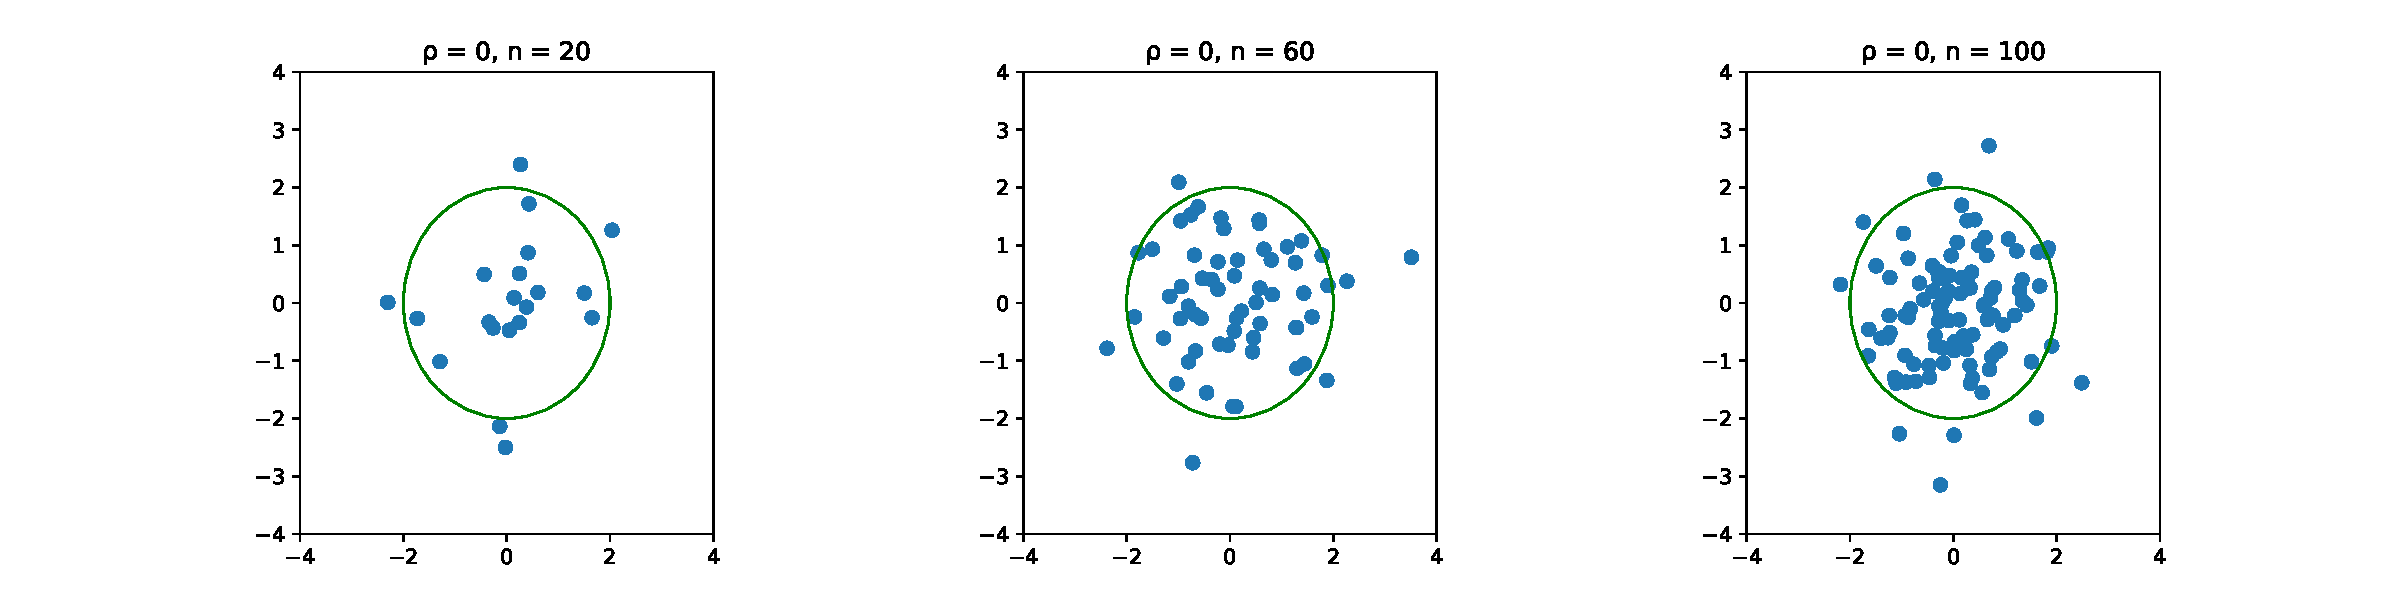
\includegraphics[width = 16cm, height = 4cm]{src_lab_5/RHO_0}
                 \caption{Двумерное нормальное распределение, $\rho$ = 0}
                 \label{fig:rho_0}
             \end{figure}

             \begin{figure}[H]
                 \centering
                 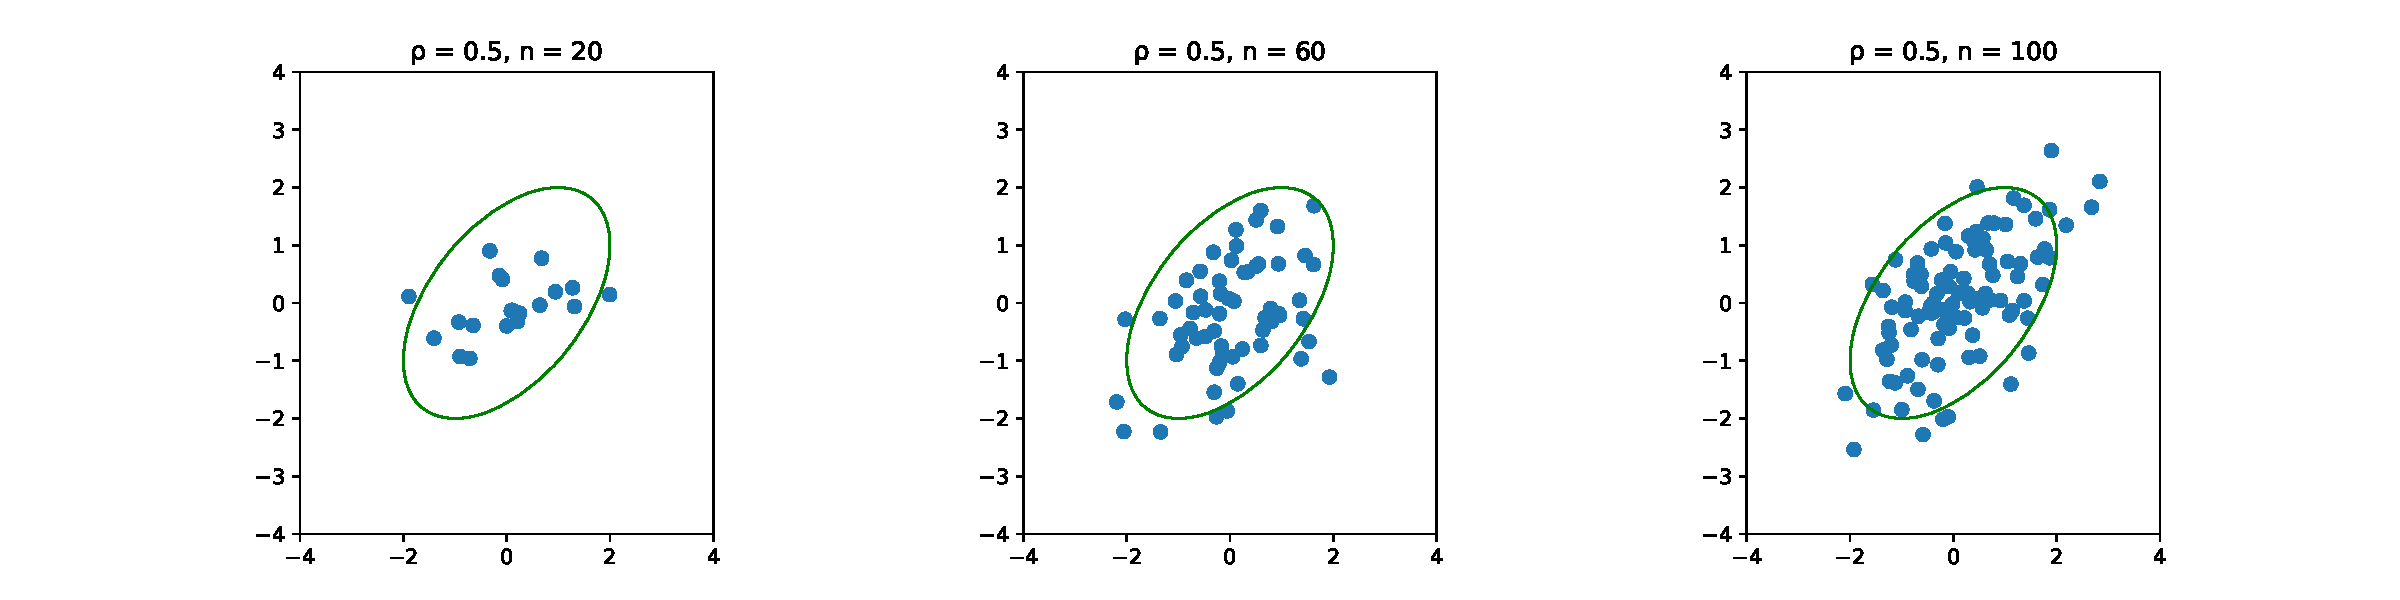
\includegraphics[width = 16cm, height = 4cm]{src_lab_5/RHO_0.5}
                 \caption{Двумерное нормальное распределение, $\rho$ = 0.5}
                 \label{fig:rho_0_5}
             \end{figure}

             \begin{figure}[H]
                 \centering
                 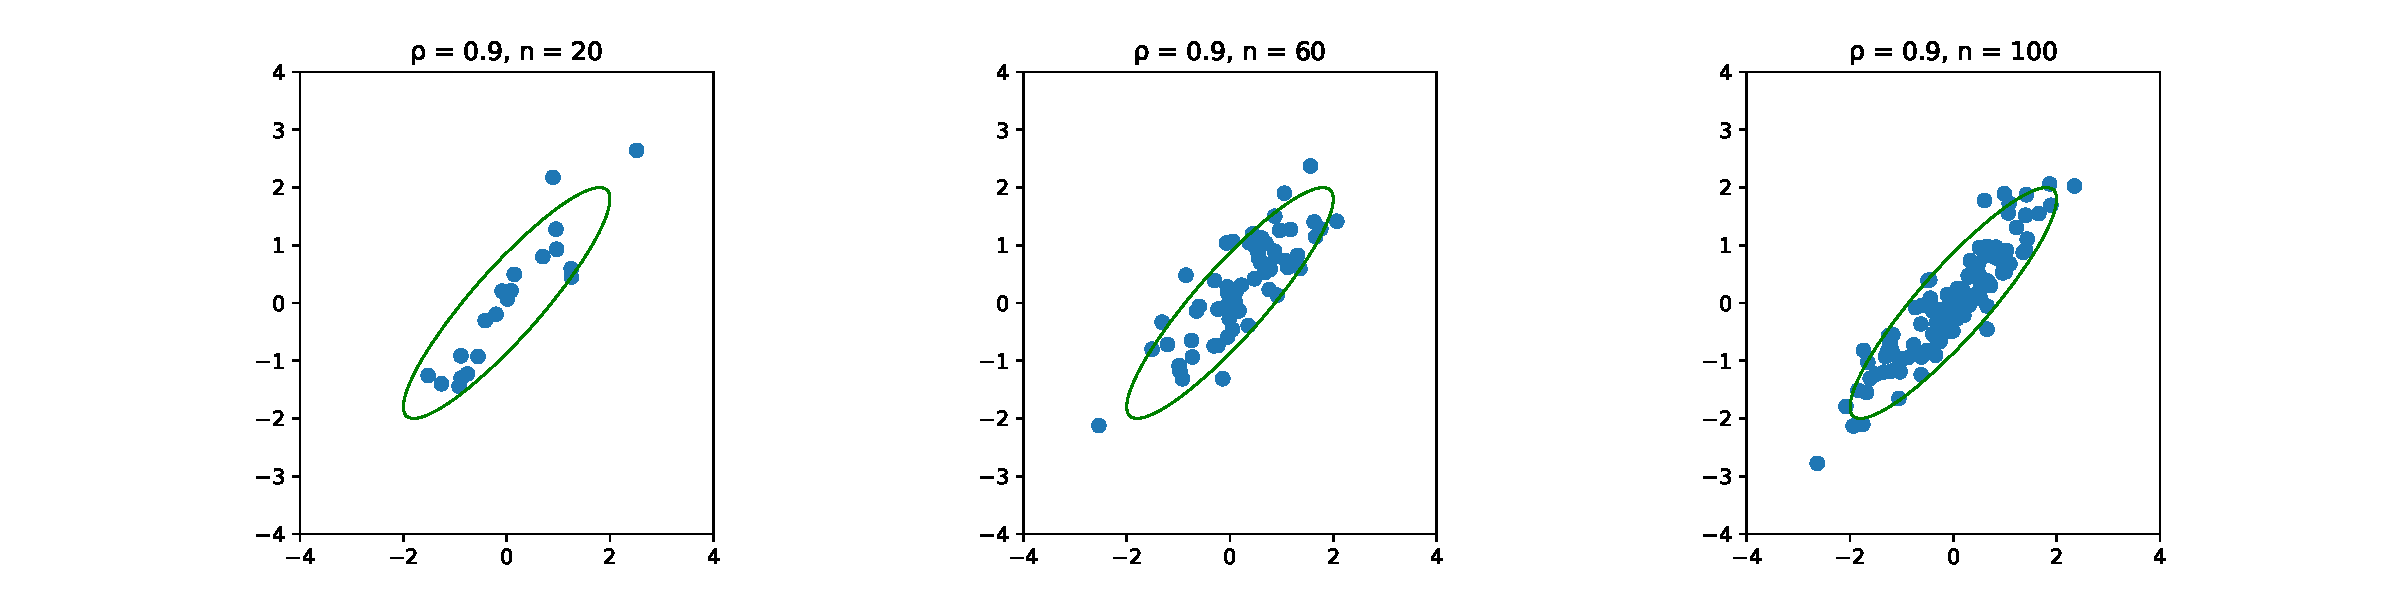
\includegraphics[width = 16cm, height = 4cm]{src_lab_5/RHO_0.9}
                 \caption{Двумерное нормальное распределение, $\rho$ = 0.9}
                 \label{fig:rho_0_9}
             \end{figure}
    \subsection{Оценки коэффициентов линейной регрессии}
            \subsubsection{Выборка без возмущений}
                \begin{enumerate}
                    \item{Критерий наименьших квадратов:}
                    $\hat{a}\approx \WithoutPertLSMBetaNULL$, $\hat{b}\approx \WithoutPertLSMBetaONE$
                    \item{Критерий наименьших модулей:}
                    $\hat{a}\approx \WithoutPertLMMBetaNULL$, $\hat{b}\approx \WithoutPertLMMBetaONE$
                \end{enumerate}
                \begin{figure}[H]
                    \centering
                    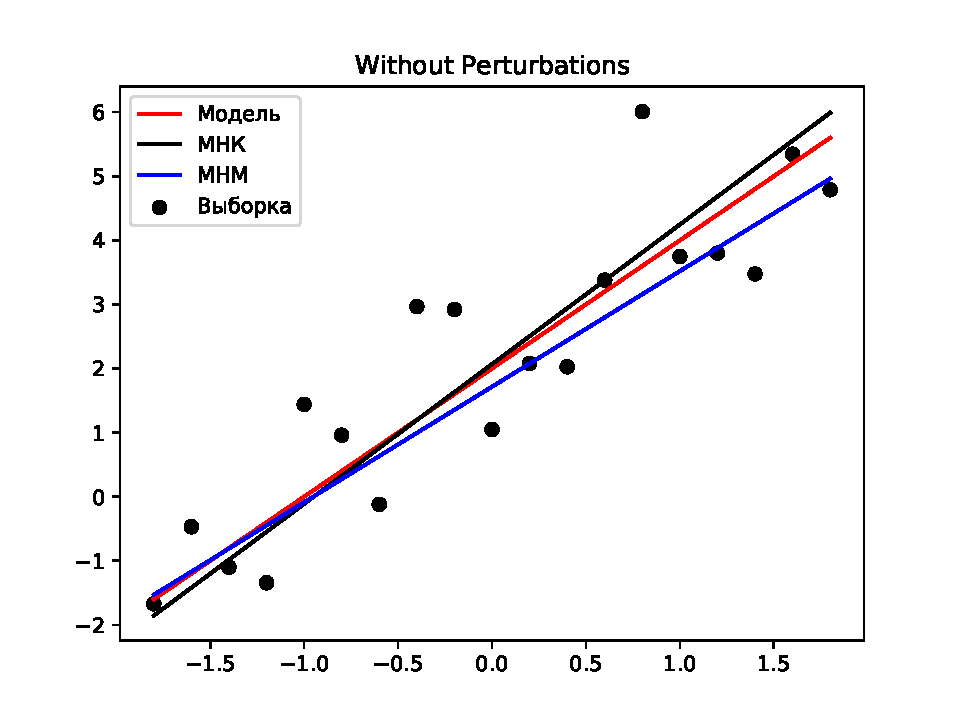
\includegraphics[width = 10cm, height = 8cm]{src_lab_6/Without Perturbations}
                    \caption{Выборка без возмущений}
                    \label{without_pert}
                \end{figure}
                МНК$~distance~=~\WithoutPertLSMDistance$ \\
		        МНМ$~distance~=~\WithoutPertLMMDistance$

            \subsubsection{Выборка с возмущениями}
                \begin{enumerate}
                    \item{Критерий наименьших квадратов:}
                    $\hat{a}\approx \WithPertLSMBetaNULL$, $\hat{b}\approx \WithPertLSMBetaONE$
                    \item{Критерий наименьших модулей:}
                    $\hat{a}\approx \WithPertLMMBetaNULL$, $\hat{b}\approx \WithPertLMMBetaONE$
                \end{enumerate}
                \begin{figure}[H]
                    \centering
                    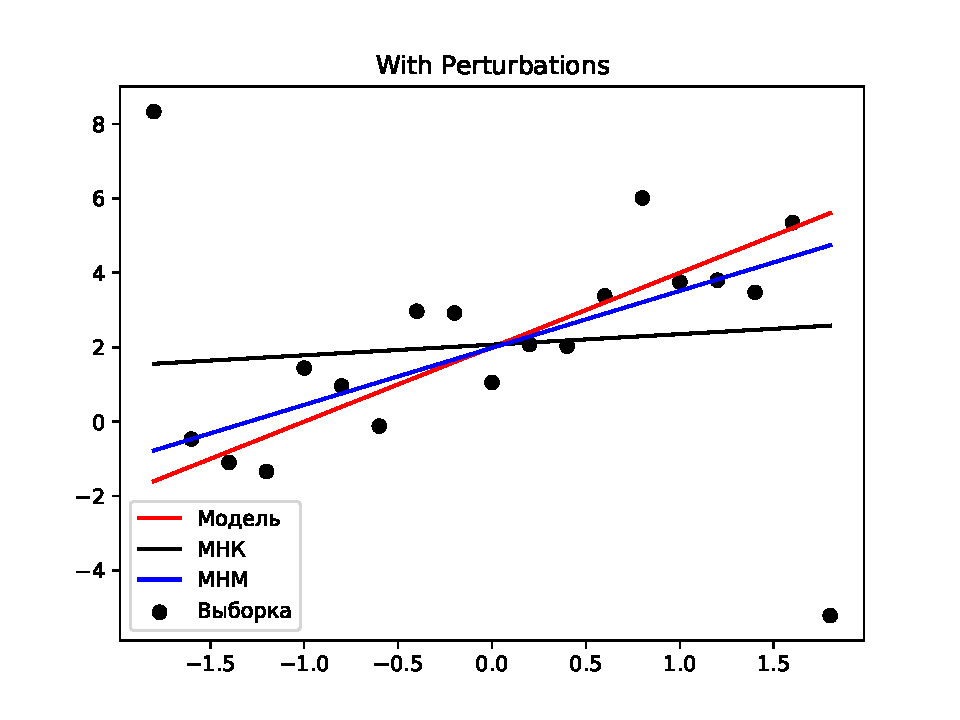
\includegraphics[width = 10cm, height = 8cm]{src_lab_6/With Perturbations}
                    \caption{Выборка с возмущениями}
                    \label{with_pert}
                \end{figure}
                МНК$~distance~=~\WithPertLSMDistance$ \\
		        МНМ$~distance~=~\WithPertLMMDistance$
    \subsection{Проверка гипотезы о законе распределения генеральной совокупности. Метод хи-квадрат}

\noindent Метод максимального правдоподобия:
\newline
$\hat{\mu} \approx -0.05, \hat{\sigma} \approx 0.95$
\newline
Критерий согласия $\chi^{2}$:
\newline
Количество промежутков $k =\BigNK$
\newline
Уровень значимости $\alpha = \LevelAlpha$
\newline
Тогда квантиль $\chi^{2}_{1-\alpha}(k-1)$ = $\chi^{2}_{0.95}(6)$$
	\newline
	\chi^{2}_{0.95}(6) \approx \BigChi$.
		\begin{table}[H]
            \centering
            \begin{tabular}{| c | c | c | c | c | c | c |}
                \hline
                i&intervals&$n_i$&$p_i$&$np_i$&$n_i - np_i$&$\dfrac{(n_i - np_i)^2}{np_i}$\\ \hline
1&[-inf, -1.1]&11&0.1357&13.5666&-2.5666&0.4856\\ \hline
2&[-1.1, -0.66]&13&0.119&11.8961&1.1039&0.1024\\ \hline
3&[-0.66, -0.22]&16&0.1583&15.8309&0.1691&0.0018\\ \hline
4&[-0.22, 0.22]&15&0.1741&17.4129&-2.4129&0.3344\\ \hline
5&[0.22, 0.66]&20&0.1583&15.8309&4.1691&1.098\\ \hline
6&[0.66, 1.1]&14&0.119&11.8961&2.1039&0.3721\\ \hline
7&[1.1, inf]&11&0.1357&13.5666&-2.5666&0.4856\\ \hline
\sum&-&100&1.0&100.0&0.0&2.8798\\ \hline

            \end{tabular}
            \caption{ Вычисление $\chi^{2}_{B}$ при проверке гипотезы $H_{0}$ о нормальном законе распределения $N(x,\hat{\mu}, \hat{\sigma})$}
			\label{tab:real_ditrib}
        \end{table}

\noindent Получили $\BigChi > \MRealDistributionChiRes$, поэтому на данном этапе гипотеза принимается.
\\
	\newline
	\newline
	Критерий согласия $\chi^{2}$:
\newline
Количество промежутков $k =\SmallNK$
\newline
Уровень значимости $\alpha = \LevelAlpha$
\newline
Тогда квантиль $\chi^{2}_{1-\alpha}(k-1)$ = $\chi^{2}_{0.95}(4)$$
	\newline
	\chi^{2}_{0.95}(6) \approx \SmallChi$.
\begin{table}[H]
	\centering
	\begin{tabular}{| c | c | c | c | c | c | c |}
		\hline
		i&intervals&$n_i$&$p_i$&$np_i$&$n_i - np_i$&$\dfrac{(n_i - np_i)^2}{np_i}$\\ \hline
1&[-inf, -1.1]&2&0.1664&3.3287&-1.3287&0.5304\\ \hline
2&[-1.1, 0.0]&5&0.3336&6.6713&-1.6713&0.4187\\ \hline
3&[0.0, 1.1]&9&0.3336&6.6713&2.3287&0.8129\\ \hline
4&[1.1, inf]&4&0.1664&3.3287&0.6713&0.1354\\ \hline
\sum&-&20&1.0&20.0&-0.0&1.8973\\ \hline

	\end{tabular}
	\caption{ Вычисление $\chi^{2}_{B}$ при проверке гипотезы $H_{0}$ о законе распределения $L(x,\hat{\mu}, \hat{\sigma})$, $n=20$}
	\label{tab:laplace_chi}
\end{table}

\noindent Получили $\SmallChi > \MLAPLACEChiRes$, поэтому на данном этапе гипотеза принимается.
\\
	\newline
	\newline
	Критерий согласия $\chi^{2}$:
\newline
Количество промежутков $k =\SmallNK$
\newline
Уровень значимости $\alpha = \LevelAlpha$
\newline
Тогда квантиль $\chi^{2}_{1-\alpha}(k-1)$ = $\chi^{2}_{0.95}(4)$$
	\newline
	\chi^{2}_{0.95}(6) \approx \SmallChi$.

\begin{table}[H]
	\centering
	\begin{tabular}{| c | c | c | c | c | c | c |}
		\hline
		i&intervals&$n_i$&$p_i$&$np_i$&$n_i - np_i$&$\dfrac{(n_i - np_i)^2}{np_i}$\\ \hline
1&[-inf, -1.1]&2&0.2381&4.7619&-2.7619&1.6019\\ \hline
2&[-1.1, 0.0]&5&0.2619&5.2381&-0.2381&0.0108\\ \hline
3&[0.0, 1.1]&9&0.2619&5.2381&3.7619&2.7017\\ \hline
4&[1.1, inf]&4&0.2381&4.7619&-0.7619&0.1219\\ \hline
\sum&-&20&1.0&20.0&0.0&4.4364\\ \hline

	\end{tabular}
	\caption{ Вычисление $\chi^{2}_{B}$ при проверке гипотезы $H_{0}$ о законе распределения $U(x,\hat{\mu}, \hat{\sigma})$, $n=20$}
	\label{tab:uniform_chi}
\end{table}

\noindent Получили $\SmallChi > \MUNIFORMChiRes$, поэтому на данном этапе гипотеза принимается.

    
	\begin{figure}[H]
		\centering
		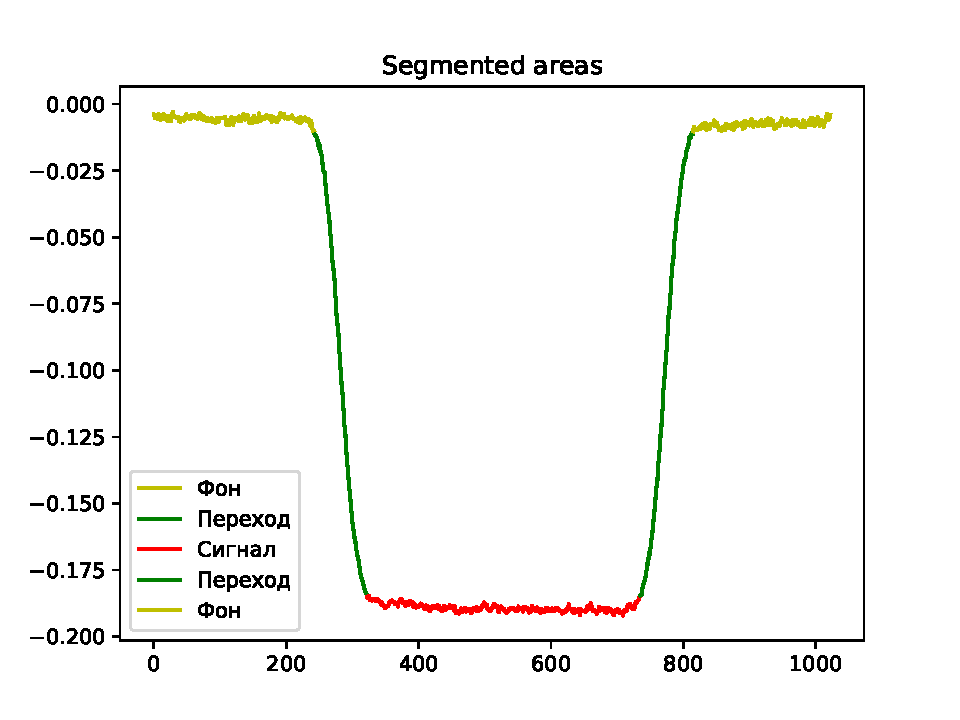
\includegraphics[width = 13cm, height = 8cm]{src_lab_8/Segmented500}
		\caption{Изображение входного сигнала}
		\label{fig:signal}
	\end{figure}

		\begin{figure}[H]
		\centering
		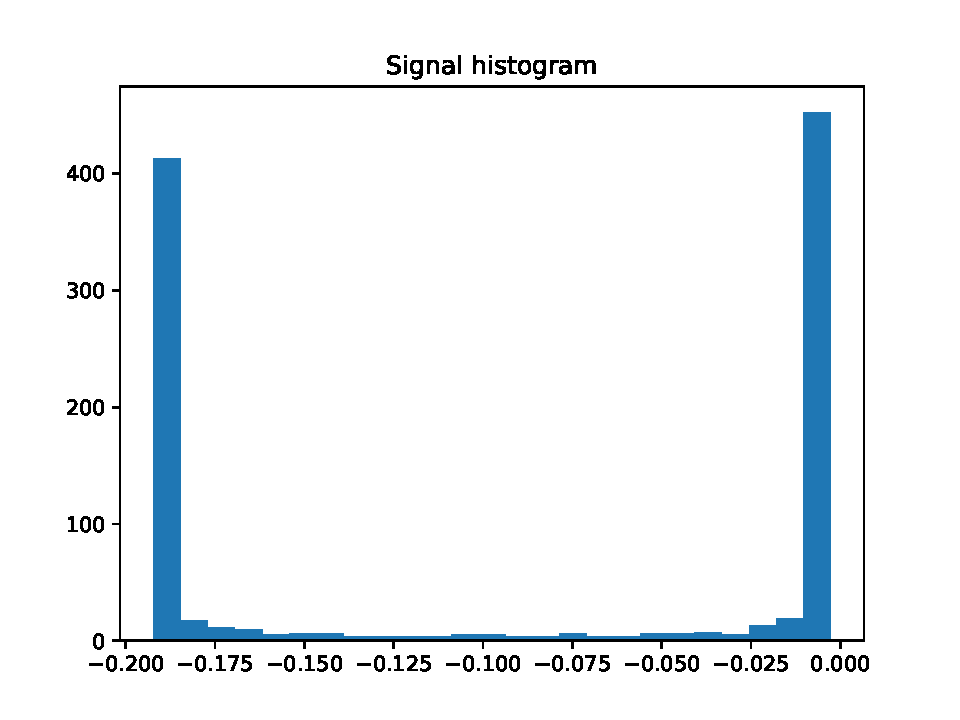
\includegraphics[width = 13cm, height = 8cm]{src_lab_8/Signal500Hist}
		\caption{Гистограмма сигнала}
		\label{fig:signalHist}
	\end{figure}

	\begin{figure}[H]
		\centering
		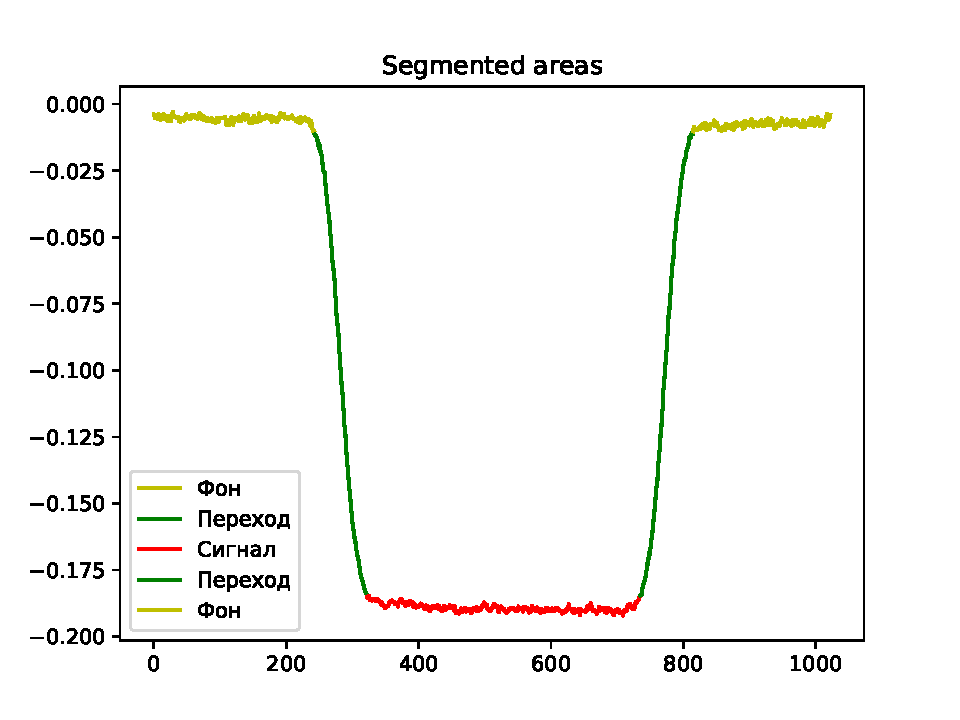
\includegraphics[width = 13cm, height = 8cm]{src_lab_8/Segmented500}
		\caption{Разделение областей для данных сигнала}
		\label{fig:signalSegmented}
	\end{figure}
	\begin{table}[H]
    \centering
    \begin{tabular}{|c|c|c|c|}
    	\hline
        Промежуток&Тип&Количество разбиений&Критерий Фишера\\ \hline
1&Фон&9&1.3668\\ \hline
2&Переход&4&19.3068\\ \hline
3&Сигнал&7&1.0187\\ \hline
4&Переход&4&19.5921\\ \hline
5&Фон&4&0.1866\\ \hline

    \end{tabular}
    \caption{Характеристики выделенных областей}
    \label{tab:FisherTab}
\end{table}
\section{Обсуждение}
\subsection{Проверка гипотезы о законе распределения генеральной совокупности. Метод хи-квадрат}

\noindent Заключаем, что гипотеза $H_{0}$ о нормальном законе распределения $N(x,\hat{\mu}, \hat{\sigma})$ на уровне значимости $\alpha = 0.05$ согласуется с выборкой для нормального распределения $N(x, 0, 1)$.
\\
Также видно, что для выборок сгенерированных по равномерному закону и закону Лапласа гипотеза $H_{0}$ оказалась принята.

\section{Приложение}
    С кодом работ и отчета можно ознакомиться по ссылке:\;\url{https://github.com/sqrtyyy/MathStat/tree/master}

\end{document}
